\section{DenseNet}
DenseNet \cite{densenet2017} was introduced in 2017. In an architecutre of this type, each layer receives ouputs from all the previous layers and then passes its input to all subsequent layers, to ensure maximum information flow.  In contrast to ResNet, where outputs are combined through summation, DenseNet uses concatenation.

Its name comes from the dense connectivity between layers. Suppose we have \textit{L} layers in the architecture. \textit{$l^{th}$} layer takes \textit{$l^{th}$} inputs (feature maps from previous layers) and its output goes to \textit{L} - \textit{$l^{th}$} following layers. This is illustrated in Figure \ref{fig:densenet}.

One of the improvements DenseNet brought, was a smaller amount of parameters to train, compared to traditional architectures or even ResNet. This feature makes it more computationally efficient. Dense layers have a few filters, which means, that the ``total'' number of feature maps passed through the network is rather small. The network then makes a decision based on all feature maps that appeared in it. Other advantages of DenseNets include memory efficiency. Furthermore, dense connections were observed to help with overfitting on small data sets.


\begin{figure}[ht!]
    \centering
    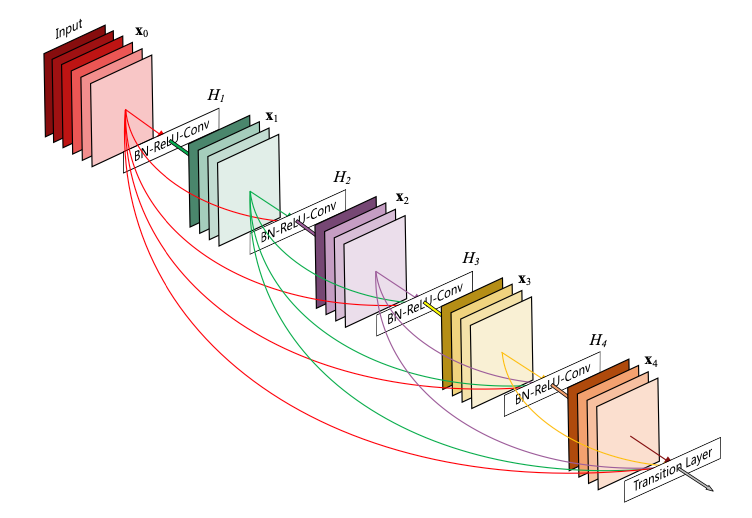
\includegraphics[width=200pt]{images/densenet.png}
    \caption[DenseNet architecture]{DenseNet architecture \cite{densenet2017}}
    \label{fig:densenet}
\end{figure}

\pagebreak